% =====================================================================
\section{Putting the Controller on the Gazebo X3 Quadcopter}
\label{sec:x3}
% =====================================================================

\subsection{Architecture}

\begin{figure}[H]
\centering
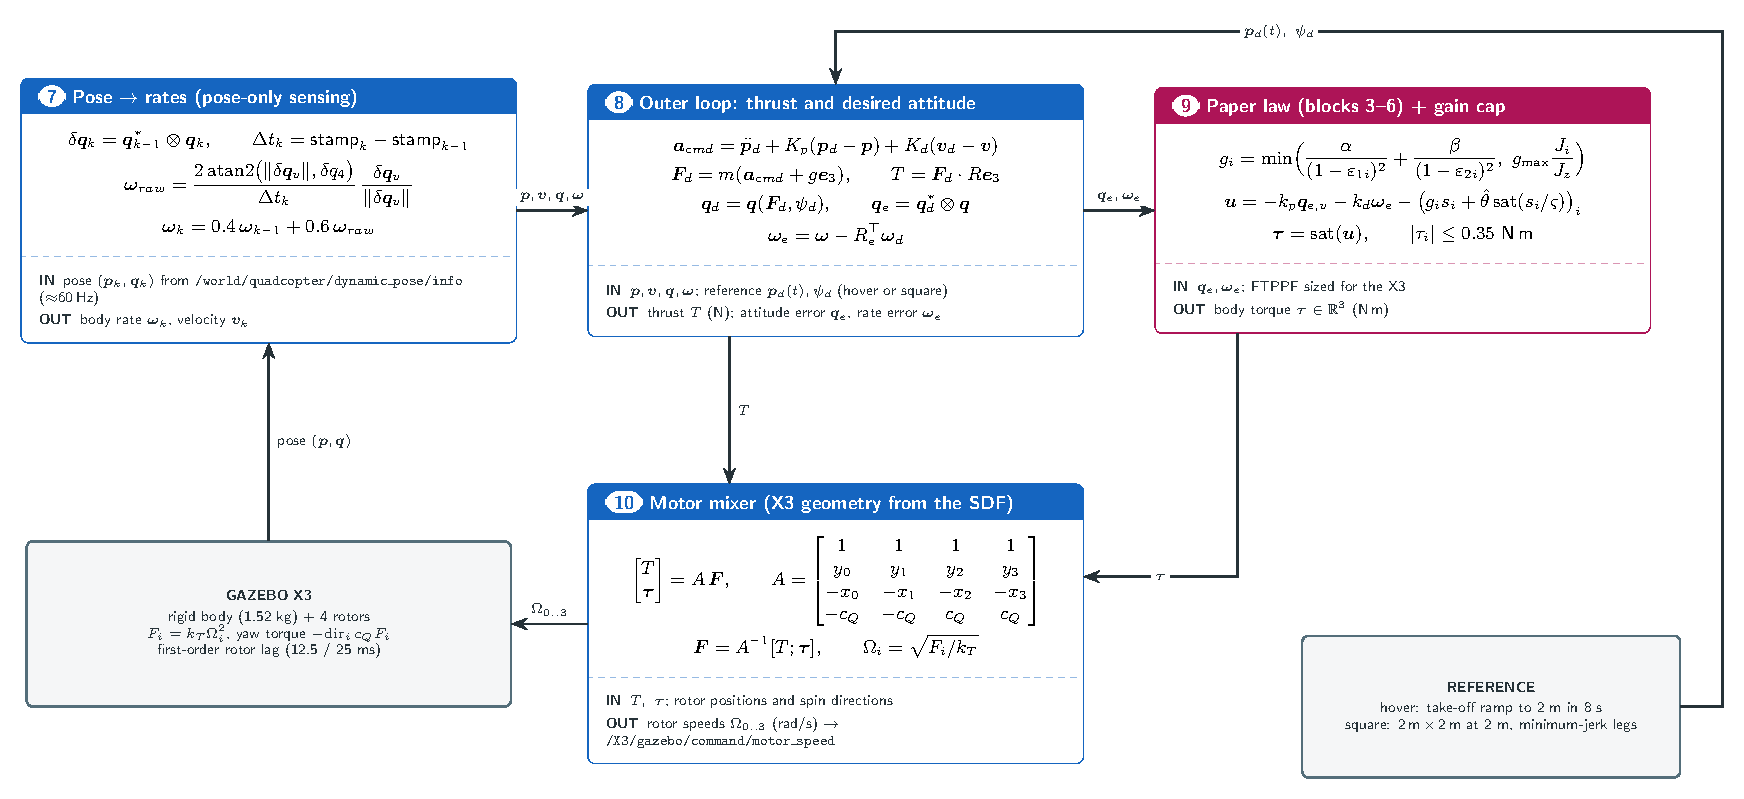
\includegraphics[width=\linewidth]{flow_x3.pdf}
\caption{Implementation flow on the X3 (Mathematical Models, Section 4). Blocks 3--6 of the paper sit inside block 9.}
\label{fig:flowx3}
\end{figure}

\begin{center}\small
\begin{tabularx}{\linewidth}{@{}l l X@{}}
\toprule
\textbf{Topic} & \textbf{Type} & \textbf{Use}\\
\midrule
\code{/world/quadcopter/dynamic\_pose/info} & \code{geometry\_msgs/PoseArray} & input: pose of the X3 with the simulation time stamp ($\approx$60\,Hz)\\
\code{/X3/gazebo/command/motor\_speed} & \code{actuator\_msgs/Actuators} & output: four rotor speeds in rad/s\\
\bottomrule
\end{tabularx}
\end{center}

\textbf{Why a software-in-the-loop surrogate.} Diagnosing a crash inside Gazebo is slow: one run per minute, no access to
the internal state, no exact repetition. We therefore wrote \code{x3\_sim/x3\_model.py}, a model of the same vehicle in
which \emph{every constant is copied from the Gazebo model files} (mass, inertia, rotor positions and spin directions,
thrust and moment constants, rotor time constants and speed limit, rotor drag), integrated with RK4 at 1\,ms, sampled at
the Gazebo pose rate of 60\,Hz with one sample of transport delay. The controller sees only what the ROS node sees: a
time stamp, a position and a quaternion. Both controllers are plain classes with the same \code{update(stamp, p, q)}
interface, so the identical code runs in the surrogate, in the offline test and inside \code{gazebo.py}.

\begin{warn}[What the surrogate does not model]
Rotor gyroscopic effects (rotor inertia is about 0.1\,\% of the body's), blade flapping, contacts other than a flat ground,
sensor noise and the ROS/Gazebo transport beyond a fixed delay. Results on the surrogate are therefore ``best case'' for
noise; Gazebo logs processed with \code{plot\_gazebo\_log.py} use the same metric definitions so the two can be compared
line by line.
\end{warn}

% ---------------------------------------------------------------------
\subsection{Why the first Gazebo node crashed}
\label{sec:x3fault}
% ---------------------------------------------------------------------

Our first node (\code{legacy/gazebo\_v1.py}) made the X3 take off and climb, then lose its attitude and crash. To find out
why without guessing, \code{OriginalGazeboController} is a line-by-line port of that node's control logic (only the ROS
plumbing removed). On the surrogate it reproduces the observed behaviour, and each suspected fault can be switched off on
its own (experiment E1).

\begin{center}\small
\begin{longtable}{@{}l p{6.0cm} p{6.6cm}@{}}
\toprule
\textbf{\#} & \textbf{Fault in v1} & \textbf{Consequence / fix in v2}\\
\midrule\endhead
F9 & Mixer signs taken from a generic ``+/$-$'' template that does not match the X3 rotor numbering. & A pitch command produced roll torque ($-0.93$ per unit), nothing produced pitch torque (\cref{tab:mixer}). Fix: exact inverse of the allocation matrix built from the SDF (block 10).\\
F10 & Yaw term divided by $c_Q$ instead of $k_Tc_Q$. & Yaw authority $10^{5}$ times too small, yaw uncontrolled. Fix: same allocation matrix.\\
F14 & \code{last\_z} set once at start and never updated. & ``Vertical speed'' $=(z-z_0)/\Delta t$ grows with height, the altitude loop cuts thrust: the drone hops and falls. Fix: update every sample.\\
F11 & Body rate from $2(\vq_k-\vq_{k-1})_v/\Delta t$ with a 0.10 filter. & Wrong axes when yawed, $\approx$150\,ms lag; slow limit cycle. Fix: $\vq_{k-1}^*\otimes\vq_k$, filter 0.6 (block 7).\\
F12 & $\Delta t$ from the wall clock (\code{time.time()}). & Timing does not match simulation time when Gazebo runs slower or faster than real time. Fix: message stamp.\\
F13 & Attitude error = raw world quaternion. & Works only for yaw 0 and no position control. Fix: $\vq_e=\vq_d^*\otimes\vq$ with an outer position loop (block 8).\\
F3 & Envelope effectively inactive ($\rho_{q0}=2$ although $|q_i|\le1$; $\alpha=\beta=0.01$; $\vu_{cons}$ clipped to 0.05\,N\,m). & The first node was in practice a plain PD. Fix: envelope and gains sized for the X3 (block 9).\\
F15 & (new in v2) unbounded barrier gain on a 60\,Hz delayed loop. & Cap $g_i\le J_i/J_z$ (block 9; MATLAB step 8).\\
\bottomrule
\end{longtable}
\end{center}

\begin{table}[H]
\centering\small
\caption{Torque produced on the X3 per unit torque commanded by the v1 mixer (ideal: identity).}
\label{tab:mixer}
\begin{tabular}{@{}lccc@{}}
\toprule
& cmd $\tau_x$ & cmd $\tau_y$ & cmd $\tau_z$\\
\midrule
produced $\tau_x$ & $+0.044$ & $\mathbf{-0.933}$ & $0$\\
produced $\tau_y$ & $0$ & $\mathbf{0}$ & $7\times10^{-5}$\\
produced $\tau_z$ & $+0.071$ & $0$ & $\mathbf{0}$\\
\bottomrule
\end{tabular}
\end{table}

The two faults in the port of v1 that matter most, next to their fixes:
\pyfile{70}{82}{\xctrl}{x3\_sim/controllers.py --- OriginalGazeboController (port of v1): z-rate and body rate}
\pyfile{113}{121}{\xctrl}{x3\_sim/controllers.py --- OriginalGazeboController (port of v1): the mixer}

\subsection{The corrected controller (v2)}

\code{FixedController} keeps the paper's law (Eq.~8, 11--14, 22) and adds blocks 7, 8, 10 and the gain cap of block 9.
\pyfile{215}{223}{\xctrl}{x3\_sim/controllers.py --- block 7: exact body rate (F11)}
\pyfile{264}{284}{\xctrl}{x3\_sim/controllers.py --- block 9: paper law with the sampled-data gain cap}
\pyfile{288}{310}{\xctrl}{x3\_sim/controllers.py --- block 10: allocation with thrust-priority de-saturation (F9, F10)}

\begin{table}[H]
\centering\small
\caption{Parameters of the paper's law: spacecraft (paper) and X3 (ours).}
\label{tab:x3params}
\begin{tabular}{@{}lcc@{}}
\toprule
\textbf{Parameter} & \textbf{Paper (spacecraft)} & \textbf{X3}\\
\midrule
inertia & $J\approx14$--$21$\,kg\,m$^2$ & $\diag(0.036,\,0.070,\,0.099)$\,kg\,m$^2$\\
torque limit & 2.5\,N\,m & 0.35\,N\,m (and rotor limits)\\
$k_p$, $k_d$ & 40, 20 & 4, 0.4\\
$\alpha$, $\beta$, $c$ & 1.5, 1.2, 0.5 & 0.15, 0.12, 1.0\\
$\eta_1$, $\eta_2$ & 0.1, $2e^{-0.5t}$ & 5, $\max(2e^{-0.5t},0.2)$, $\that\le0.1$\\
$\varsigma$ & 0.02 & 0.5\\
$\rho_q$: $\rho_0\to\rho_T$ & $0.3\to0.008$ & $0.30\to0.02$\\
$\rho_\omega$: $\rho_0\to\rho_T$ & $0.4\to0.005$\,rad/s & $2.5\to0.05$\,rad/s\\
$\kappa$, $T_s$ & 2.5, 10--15\,s & 2, 10\,s\\
natural frequency, damping (PD part) & 1.08\,rad/s, 0.54 & 7.5\,rad/s, 0.75 (roll)\\
barrier gain cap & none & $g_i\le J_i/J_z$ (0.36, 0.71, 1.0)\\
\bottomrule
\end{tabular}
\end{table}

\subsection{The ROS~2 node}

\code{gazebo.py} (v2) is a thin wrapper: it reads the pose and the \emph{message stamp}, calls the
\code{update()} method of \code{FixedController}, publishes the four rotor speeds, optionally injects the paper's disturbance as an extra
body torque through the rotors, logs everything and stops after the chosen duration. The experiment, controller and
disturbance are ROS parameters (\cref{sec:setup}). The offline test drives the real node file, with \code{rclpy} and the
two message types replaced by minimal stand-ins, against the surrogate at 60\,Hz with one sample of delay.

\begin{projbox}[offline test of the node (\code{tests/test\_gazebo\_node\_offline.py})]
Hover, 40\,s: final position $(0.000,\ 0.000,\ 2.000)$\,m. Square, 45\,s: returns to $(0.000,\ 0.000,\ 2.000)$\,m. Hover with
$0.5\times$ the paper's disturbance injected through the rotors (symmetric barrier): final position $(0.030,\ 0.056,\ 2.000)$\,m.
The log is processed by \code{plot\_gazebo\_log.py} without error. Result: \code{ALL OFFLINE NODE TESTS PASSED}.
\end{projbox}
